\PassOptionsToPackage{unicode=true}{hyperref} % options for packages loaded elsewhere
\PassOptionsToPackage{hyphens}{url}
%
\documentclass[12pt,]{article}
\usepackage{lmodern}
\usepackage{amssymb,amsmath}
\usepackage{ifxetex,ifluatex}
\usepackage{fixltx2e} % provides \textsubscript
\ifnum 0\ifxetex 1\fi\ifluatex 1\fi=0 % if pdftex
  \usepackage[T1]{fontenc}
  \usepackage[utf8]{inputenc}
  \usepackage{textcomp} % provides euro and other symbols
\else % if luatex or xelatex
  \usepackage{unicode-math}
  \defaultfontfeatures{Ligatures=TeX,Scale=MatchLowercase}
    \setmainfont[]{Times New Roman}
\fi
% use upquote if available, for straight quotes in verbatim environments
\IfFileExists{upquote.sty}{\usepackage{upquote}}{}
% use microtype if available
\IfFileExists{microtype.sty}{%
\usepackage[]{microtype}
\UseMicrotypeSet[protrusion]{basicmath} % disable protrusion for tt fonts
}{}
\IfFileExists{parskip.sty}{%
\usepackage{parskip}
}{% else
\setlength{\parindent}{0pt}
\setlength{\parskip}{6pt plus 2pt minus 1pt}
}
\usepackage{hyperref}
\hypersetup{
            pdftitle={Analysis of arsenic and PFAS occurrence in United States community water systems},
            pdfauthor={Rachel Gonsenhauser},
            pdfborder={0 0 0},
            breaklinks=true}
\urlstyle{same}  % don't use monospace font for urls
\usepackage[margin=2.54cm]{geometry}
\usepackage{longtable,booktabs}
% Fix footnotes in tables (requires footnote package)
\IfFileExists{footnote.sty}{\usepackage{footnote}\makesavenoteenv{longtable}}{}
\usepackage{graphicx,grffile}
\makeatletter
\def\maxwidth{\ifdim\Gin@nat@width>\linewidth\linewidth\else\Gin@nat@width\fi}
\def\maxheight{\ifdim\Gin@nat@height>\textheight\textheight\else\Gin@nat@height\fi}
\makeatother
% Scale images if necessary, so that they will not overflow the page
% margins by default, and it is still possible to overwrite the defaults
% using explicit options in \includegraphics[width, height, ...]{}
\setkeys{Gin}{width=\maxwidth,height=\maxheight,keepaspectratio}
\setlength{\emergencystretch}{3em}  % prevent overfull lines
\providecommand{\tightlist}{%
  \setlength{\itemsep}{0pt}\setlength{\parskip}{0pt}}
\setcounter{secnumdepth}{5}
% Redefines (sub)paragraphs to behave more like sections
\ifx\paragraph\undefined\else
\let\oldparagraph\paragraph
\renewcommand{\paragraph}[1]{\oldparagraph{#1}\mbox{}}
\fi
\ifx\subparagraph\undefined\else
\let\oldsubparagraph\subparagraph
\renewcommand{\subparagraph}[1]{\oldsubparagraph{#1}\mbox{}}
\fi

% set default figure placement to htbp
\makeatletter
\def\fps@figure{htbp}
\makeatother

\usepackage{etoolbox}
\makeatletter
\providecommand{\subtitle}[1]{% add subtitle to \maketitle
  \apptocmd{\@title}{\par {\large #1 \par}}{}{}
}
\makeatother

\title{Analysis of arsenic and PFAS occurrence in United States community water
systems}
\providecommand{\subtitle}[1]{}
\subtitle{\url{https://github.com/rachel-gonsenhauser/Final_Project_Environmental_Data_Analytics}}
\author{Rachel Gonsenhauser}
\date{}

\begin{document}
\maketitle

\newpage
\abstract

While the Safe Drinking Water Act seeks to establish standards for many
drinking water contaminants, many water systems still experience
elevated concentrations of contaminants. This analysis compares arsenic
concentrations in southeastern and northeastern states, explores whether
the occurrence of other water contaminants and choosen socioeconomic
factors predict arsenic concentrations in North Carolina and
Massachusetts, and examines whether socioeconomic factors explain
variation in PFAS concentrations in the United States. Results indicate
that North Carolina and South Carolina experience elevated arsenic
concentrations compared to other southeastern states, as do
Massachusetts and Maine as compared to other northeastern states.
Arsenic concentrations are significantly predicted by trihaloomethane
concentrationos and by size of the population served by a Community
Water System (CWS) in North Carolina but not in Massachusetts. Finally,
socioeconomic variables examined do not siginficanntly explain variation
inn PFAS concentrations.

\newpage
\tableofcontents 
\newpage
\listoftables 
\newpage
\listoffigures 
\newpage

\hypertarget{rationale-and-research-questions}{%
\section{Rationale and Research
Questions}\label{rationale-and-research-questions}}

While the EPA establishes standards for 90 drinking water contaminants
by means of the federal Safe Drinking Water Act (SDWA) and its
regulations, public water systems still often struggle to remain in
compliance with such policies (``Safe Drinking Water Act (SDWA)'',
2020). This issue of compliance with the SDWA can stem from myriad
causes, for instance financial capacity of the water system. This is
especially concerning in areas where geologic conditions and/or
anthropogenic activities frequently introduce contaminants into drinking
water supplies. Additionally, some known contaminants still have yet to
be regulated by the EPA, such as poly- and perfluoroaklyl substances
(PFAS), which introduces even more complexity to the issue of water
quality monitoring of drinking water sources.

This analysis seeks to investigate the co-occurrence of water quality
indicators including arsenic, trihalomethane, uranium, and PFAS, which
originate from both geogenic and anthropogenic sources. Additionally,
given pervasive questions about how socioeconomic factors may be related
to water quality indicators, this analysis seeks to examine
relationships between water quality indicators and county-level median
household income (MHI) and size of the population served by a given
community water system (CWS). Additionally, questions regarding how
contaminant occurrences differ between states are explored.

To narrow the scope of this project, most analyses are targeted to
southeastern region states and northeastern region states. These regions
were chosen given their differences in climate, geology, and demographic
makeup. Additionally, individual case studies of Massachusetts and North
Carolina, selected following the data exploration phase, are explored in
further depth.

As arsenic is present in much of the underlying geology in many states
in both the northeast and southeast, arsenic concentration data is
predominant focus of most analyses performed. Given that PFAS are
emerging, synthetic contaminants that have become the focus of many
analyses in the scientific community, PFAS data is also explored in
depth. Due to data limitations however, discussed in more detail in the
subsequent section, analyses using PFAS data herein are limited.

Specifically, the subsequent analysis explores the following questions:
-\textbf{Question 1:} Do arsenic concentrations vary significantly from
state to state in northeastern and southeastern states?
-\textbf{Question 2:} Do socioeconomic factors or the presence of other
contaminants predict arsenic concentrations in Massachusetts and North
Carolina? -\textbf{Question 3.} Are socioeconomic factors significant
predictors of PFAS concentrations?

\newpage

\hypertarget{dataset-information}{%
\section{Dataset Information}\label{dataset-information}}

Data used for this analysis was downloaded from the Centers for Disease
Control and Prevention (CDC)'s National Environmental Public Health
Tracking Network at Centers for Disease Control and Prevention (CDC)'s
National Environmental Public Health Tracking Network
\url{https://ephtracking.cdc.gov/DataExplorer/\#/}. Output from this
online tool containing geographic and CWS data associated with
individual variables was combined into the final processed dataset used
for this analysis.

The wrangling process entailed taking individual datasets containing
data for arsenic, PFAS, uranium, trihalomethane, and MHI and joining
them into the final processed dataset. Each of these variables had
accompanying data inncluding the year, state, county, and CWS in which
the data was collected for each parameter. As unique county Federal
Information Processing Standards (FIPS) codes were standard across all
individual datasets, this variable was used to join datasets into the
final processed dataset.

Figure 1: Summary information for processed dataset

\begin{longtable}[]{@{}ll@{}}
\toprule
\textbf{Parameter} & \textbf{Summary}\tabularnewline
\midrule
\endhead
Number of states & 28\tabularnewline
Number of CWSs & 25,583\tabularnewline
Water quality indicators & Arsenic, trihalomethane, uranium,
PFAS\tabularnewline
Socioeconomic variables & Population served by CWS, MHI\tabularnewline
Data collection time span & 1999-2018\tabularnewline
\bottomrule
\end{longtable}

Figure 2: Description of Variables Used in Analyses

\begin{longtable}[]{@{}lll@{}}
\toprule
\begin{minipage}[b]{0.22\columnwidth}\raggedright
\textbf{Column Heading}\strut
\end{minipage} & \begin{minipage}[b]{0.46\columnwidth}\raggedright
\textbf{Variable Description}\strut
\end{minipage} & \begin{minipage}[b]{0.23\columnwidth}\raggedright
\textbf{Data Range}\strut
\end{minipage}\tabularnewline
\midrule
\endhead
\begin{minipage}[t]{0.22\columnwidth}\raggedright
stateFIPS\strut
\end{minipage} & \begin{minipage}[t]{0.46\columnwidth}\raggedright
Federal Information Processing Standard state code\strut
\end{minipage} & \begin{minipage}[t]{0.23\columnwidth}\raggedright
N/A\strut
\end{minipage}\tabularnewline
\begin{minipage}[t]{0.22\columnwidth}\raggedright
State\strut
\end{minipage} & \begin{minipage}[t]{0.46\columnwidth}\raggedright
state measurement was taken in\strut
\end{minipage} & \begin{minipage}[t]{0.23\columnwidth}\raggedright
N/A\strut
\end{minipage}\tabularnewline
\begin{minipage}[t]{0.22\columnwidth}\raggedright
countyFIPS\strut
\end{minipage} & \begin{minipage}[t]{0.46\columnwidth}\raggedright
Federal Information Processing Standard county code\strut
\end{minipage} & \begin{minipage}[t]{0.23\columnwidth}\raggedright
N/A\strut
\end{minipage}\tabularnewline
\begin{minipage}[t]{0.22\columnwidth}\raggedright
County\strut
\end{minipage} & \begin{minipage}[t]{0.46\columnwidth}\raggedright
county measurement was taken in\strut
\end{minipage} & \begin{minipage}[t]{0.23\columnwidth}\raggedright
N/A\strut
\end{minipage}\tabularnewline
\begin{minipage}[t]{0.22\columnwidth}\raggedright
Year\strut
\end{minipage} & \begin{minipage}[t]{0.46\columnwidth}\raggedright
year measurement was taken in\strut
\end{minipage} & \begin{minipage}[t]{0.23\columnwidth}\raggedright
N/A\strut
\end{minipage}\tabularnewline
\begin{minipage}[t]{0.22\columnwidth}\raggedright
Arsenic\_ugL\strut
\end{minipage} & \begin{minipage}[t]{0.46\columnwidth}\raggedright
mean arsenic concentration (micrograms per liter)\strut
\end{minipage} & \begin{minipage}[t]{0.23\columnwidth}\raggedright
1-2,422 micrograms/liter\strut
\end{minipage}\tabularnewline
\begin{minipage}[t]{0.22\columnwidth}\raggedright
PWS.ID\strut
\end{minipage} & \begin{minipage}[t]{0.46\columnwidth}\raggedright
Public Water System Identification Number\strut
\end{minipage} & \begin{minipage}[t]{0.23\columnwidth}\raggedright
N/A\strut
\end{minipage}\tabularnewline
\begin{minipage}[t]{0.22\columnwidth}\raggedright
CWS.Name\strut
\end{minipage} & \begin{minipage}[t]{0.46\columnwidth}\raggedright
Community Water System Name\strut
\end{minipage} & \begin{minipage}[t]{0.23\columnwidth}\raggedright
N/A\strut
\end{minipage}\tabularnewline
\begin{minipage}[t]{0.22\columnwidth}\raggedright
Population.Served\strut
\end{minipage} & \begin{minipage}[t]{0.46\columnwidth}\raggedright
number of people served by CWS\strut
\end{minipage} & \begin{minipage}[t]{0.23\columnwidth}\raggedright
0-8,271,000 people\strut
\end{minipage}\tabularnewline
\begin{minipage}[t]{0.22\columnwidth}\raggedright
MHI\strut
\end{minipage} & \begin{minipage}[t]{0.46\columnwidth}\raggedright
median household income (\$)\strut
\end{minipage} & \begin{minipage}[t]{0.23\columnwidth}\raggedright
\$16,435-\$113,336\strut
\end{minipage}\tabularnewline
\begin{minipage}[t]{0.22\columnwidth}\raggedright
PFAS\_ppt\strut
\end{minipage} & \begin{minipage}[t]{0.46\columnwidth}\raggedright
PFAS conncentration (parts per trillion)\strut
\end{minipage} & \begin{minipage}[t]{0.23\columnwidth}\raggedright
1-60 ppt\strut
\end{minipage}\tabularnewline
\begin{minipage}[t]{0.22\columnwidth}\raggedright
TTHM\_ugl\strut
\end{minipage} & \begin{minipage}[t]{0.46\columnwidth}\raggedright
mean trihalomethane concentration (micrograms per liter)\strut
\end{minipage} & \begin{minipage}[t]{0.23\columnwidth}\raggedright
0-219.20 micrograms/liter\strut
\end{minipage}\tabularnewline
\begin{minipage}[t]{0.22\columnwidth}\raggedright
Uranium\_ugL\strut
\end{minipage} & \begin{minipage}[t]{0.46\columnwidth}\raggedright
mean uranium concentration (micrograms per liter)\strut
\end{minipage} & \begin{minipage}[t]{0.23\columnwidth}\raggedright
0-379.10 micrograms/liter\strut
\end{minipage}\tabularnewline
\begin{minipage}[t]{0.22\columnwidth}\raggedright
MCL\_TTM\strut
\end{minipage} & \begin{minipage}[t]{0.46\columnwidth}\raggedright
whether MCL for trihalomethanes is exceeded\strut
\end{minipage} & \begin{minipage}[t]{0.23\columnwidth}\raggedright
N/A\strut
\end{minipage}\tabularnewline
\begin{minipage}[t]{0.22\columnwidth}\raggedright
MCL\_Uranium\strut
\end{minipage} & \begin{minipage}[t]{0.46\columnwidth}\raggedright
whether MCL for uranium is exceeded\strut
\end{minipage} & \begin{minipage}[t]{0.23\columnwidth}\raggedright
N/A\strut
\end{minipage}\tabularnewline
\begin{minipage}[t]{0.22\columnwidth}\raggedright
MCL\_Arsenic\strut
\end{minipage} & \begin{minipage}[t]{0.46\columnwidth}\raggedright
whether MCL for arsenic is exceeded\strut
\end{minipage} & \begin{minipage}[t]{0.23\columnwidth}\raggedright
N/A\strut
\end{minipage}\tabularnewline
\bottomrule
\end{longtable}

Table 1 provides a high level summary of the data provided in the
processed dataset. It should be noted that PFAS data was only available
for 2013-2015. For ease of analysis, this date range was changed to 2014
during the raw dataset wrangling process to create a common annual unit
of analysis for all variables. Table 2 provides descriptions of all
variables included in the processed dataset with data ranges provided
for continuous variables.

\newpage

\hypertarget{exploratory-analysis}{%
\section{Exploratory Analysis}\label{exploratory-analysis}}

While the distributions of all variables in the dataset were explored
during data wrangling and exploration, this section highlights key
results from the data exploration process. As research questions focus
on arsenic and PFAS concentrations, this exploratory analysis will
primarly explore data for these two variables.

\hypertarget{data-exploration-for-southeastern-states}{%
\subsection{Data Exploration for Southeastern
States}\label{data-exploration-for-southeastern-states}}

Table 3: Summary Statistics for Southeastern State Variables

\begin{longtable}[]{@{}lll@{}}
\toprule
\textbf{Parameter} & \textbf{Mean} & \textbf{Data Range}\tabularnewline
\midrule
\endhead
MHI & \$40,848 & \$16,435-\$92,097\tabularnewline
Population served by CWS & 14,893 people & 0-2,300,000
people\tabularnewline
Arsenic & 410.6 micrograms/liter & 1.0-2,395.0
micrograms/liter\tabularnewline
Uranium & 0.681 micrograms/liter & 0-23.84
micrograms/liter\tabularnewline
PFAS & 31.71 ppt & 7.0-59.00 ppt\tabularnewline
Trihalomethane & 17.47 micrograms/liter & 0-80.00
micrograms/liter\tabularnewline
\bottomrule
\end{longtable}

Southeastern states examined include counties with a large range of
income levels and water system sizes; additionally, arsenic
concentrations vary more than any other contaminant examined (Table 3).

\begin{figure}
\centering
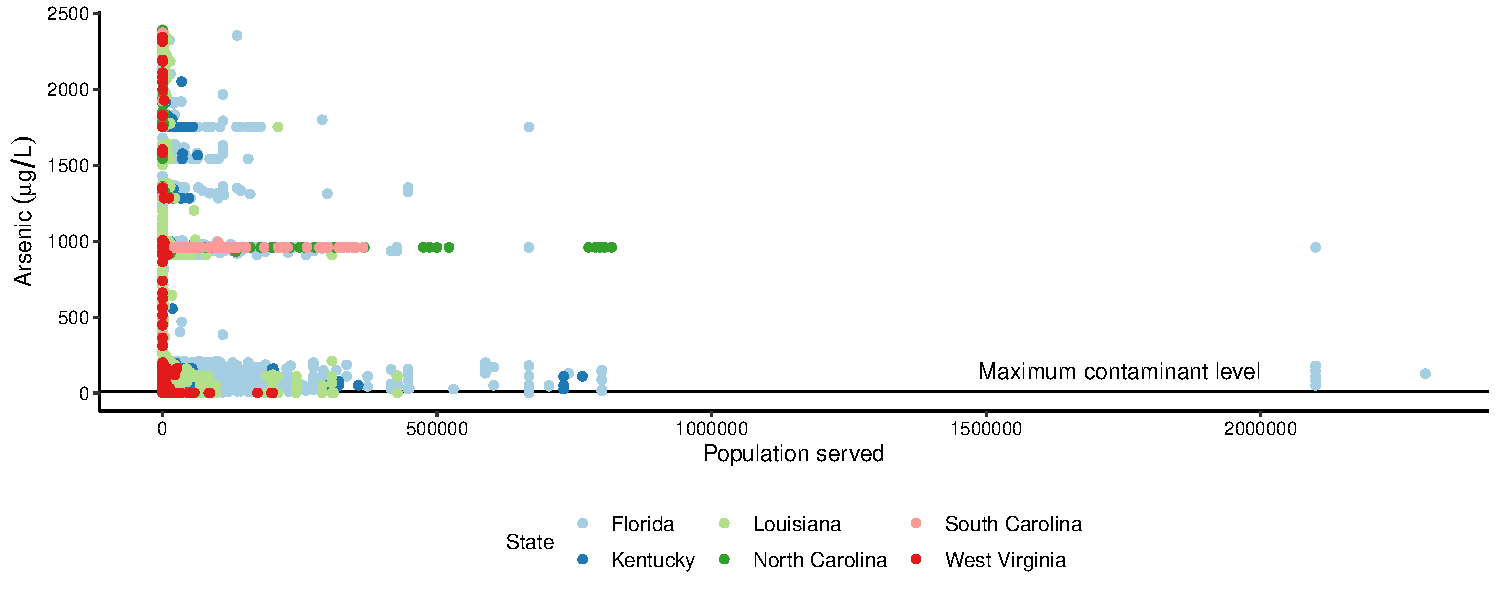
\includegraphics{Project_Template_files/figure-latex/figs-1.pdf}
\caption{Frequency of Arsenic Concentration Data in Southeastern
states.}
\end{figure}

West Virginia, Florida, Louisiana, and Kentucky all have relatively high
counts of arsenic observations at low concentration levels (Figure 1).
At the same time, North Carolina, South Carolina, and Florida have
relatively high counts of arsenic observations at higher concentrations
(around 1,000 micrograms/liter). This exploration of arsenic data in
southeastern states justifies an examination of how arsenic
concentrations vary among southeastern states and which explanatory
variables might predict arsenic concentrations.

\begin{figure}
\centering
\includegraphics{Project_Template_files/figure-latex/figs2-1.pdf}
\caption{Frequency of PFAS Concentration Data in Southeastern states.}
\end{figure}

Compared to arsenic data, PFAS concentration data is far more limited in
southeastern states (Figure 2). The largest frequency of counts occurs
in Florida at around 45 ppt with only two counts available. This
limitation of data on PFAS concentrations justifies a separate analysis
of PFAS data at a nationwide scale as examining PFAS data regionally
severely limits the availability of data.

\newpage

\hypertarget{data-exploration-for-northeastern-states}{%
\subsection{Data Exploration for Northeastern
States}\label{data-exploration-for-northeastern-states}}

Table 3: Summary Statistics for Northeastern State Variables

\begin{longtable}[]{@{}lll@{}}
\toprule
\textbf{Parameter} & \textbf{Mean} & \textbf{Data Range}\tabularnewline
\midrule
\endhead
MHI & \$54,513 & \$26,323-\$113,336\tabularnewline
Population served by CWS & 13,791 people & 0-8,271,000
people\tabularnewline
Arsenic & 359.2 micrograms/liter & 1.0-2,2,422.0
micrograms/liter\tabularnewline
Uranium & 1.75 micrograms/liter & 0-43.00
micrograms/liter\tabularnewline
PFAS & 29.76 ppt & 3-60.00 ppt\tabularnewline
Trihalomethane & 10.37 micrograms/liter & 0-134.10
micrograms/liter\tabularnewline
\bottomrule
\end{longtable}

Summary statistics for the northeastern United States indicate the the
median household income is higher than that in the southeast and that
while the average water system size is similar across regions, the
northeast has systems to serve upwards of 8 million people, as compared
to a maxiumum size of 2 million people in the southeast (Tables 3 and
4). Ranges and average values for water quality indicators were
relatively similar in both regions (Tables 3 and 4).

\begin{figure}
\centering
\includegraphics{Project_Template_files/figure-latex/figs3-1.pdf}
\caption{Frequency of Arsenic Concentration Data in Noutheastern
states.}
\end{figure}

All northeastn states appear to have relatively high counts of arsenic
observations at low concentration levels, with New York and Pennsylvania
maintaining the highest counts (Figure 3). Additionally, Massachusetts,
New York, and Connecticut, among other states also have many
observations at elevated arsenic concentrations (around 1,000
micrograms/liter). Similarly to southeastern states, the exploration of
arenic data in northeastern states justifies a comparison of arsenic
concentrations across northeastern states. Additionally, understanding
which explanatory variables predict arsenic concentrations, particularly
in states with elevated levels, will be explored in the subsequent
analysis performed.

\newpage

\begin{figure}
\centering
\includegraphics{Project_Template_files/figure-latex/figs4-1.pdf}
\caption{Frequency of PFAS Concentration Data in Noutheastern states.}
\end{figure}

Much like in southeastern states, PFAS concentration data in
northeastern states is very limited (Figure 4). The largest frequency of
counts occurs in New Jersey at around 38 ppt with only two counts
available. Again, this data limitation provides rationale for examining
PFAS data on a nationwide scale, rather than regionally, which will be
conducted in the subsequent analysis.

\newpage

\hypertarget{case-studies-data-exploration-for-north-carolina-and-massachusetts}{%
\subsection{Case Studies: Data Exploration for North Carolina and
Massachusetts}\label{case-studies-data-exploration-for-north-carolina-and-massachusetts}}

North Carolina and Massachusetts were selected as individual case
studies due to the prevalence of arsenic data at high concentrations
revealed earlier in the exploratory analysis. To gain insight into how
arsenic concentrations vary with respect to the variation of other
contaminants, arsenic, uranium, and trihalomethane data are provided
below across the data collection time span (1999-2018).

\begin{figure}
\centering
\includegraphics{Project_Template_files/figure-latex/figs5-1.pdf}
\caption{Water contaminant concentrations over time in North Carolina.}
\end{figure}

Over the period of 1999-2018 examined, North Carolina experiences
consistent levels of arsenic, uranium, and trihalomethane (Figure 5).
The maximum cotaminant levels (MCL) for these three contaminants, set by
the US EPA, are 10 micrograms/liter, 30 micograms/liter, and 80
micrograms/liter respectively. As such, uranium and trihalomethane
concentrations in North Carolina over this period of time remain safely
below the MCL standard. Arsenic concentrations, on the other hand,
appear to occur well above the MCL for the entire period of time
examined.

\newpage

\begin{figure}
\centering
\includegraphics{Project_Template_files/figure-latex/figs6-1.pdf}
\caption{Water contaminant concentrations over time in Massachusetts.}
\end{figure}

Over the same period of time, Massachusetts experiences slightly
declining arsenic concentrations, substantially declining uranium
concentrations, and relatively constant trihalomethaen concentrations
(Figure 6). Trihalomethane concentrations are safely below the MCL
standard, as are uranium concentrations from about 2010-2018.
Conversely, arsenic concentrations remain high over the entire 19-year
time span examined.

This exploratory analysis has highlighted that arsenic concentrations
likely vary among states in the southeast and northeast and that
elevated arsenic levels occur in both North Carolina and Massachusetts.
As such, the subsequent analysis will focus primarily on examining
arsenic concentrations. Additionally, limited PFAS data highlighted
during this data exploration process motivates a separate analysis of
PFAS data during the analysis phase.

\newpage

\hypertarget{analysis}{%
\section{Analysis}\label{analysis}}

The following analysis seeks to answer the three questions stated at the
onset of this report. Key results of statistical analyses performed will
be provided below.

\hypertarget{question-1-do-arsenic-concentrations-vary-significantly-from-state-to-state-in-northeastern-and-southeastern-states}{%
\subsection{Question 1: Do arsenic concentrations vary significantly
from state to state in northeastern and southeastern
states?}\label{question-1-do-arsenic-concentrations-vary-significantly-from-state-to-state-in-northeastern-and-southeastern-states}}

\begin{figure}
\centering
\includegraphics{Project_Template_files/figure-latex/figs7-1.pdf}
\caption{State by state comparison of arsenic values for southeastern
states.}
\end{figure}

Mean annual arsenic concentrations differ significantly between states
in the southeast (ANOVA; df=5, F=2872, p \textless{}0.0001). Mean
arsenic concentrations in West Virginia were significantly lower than in
other states and those in North Carolina and South Carolina were
significantly higher than those in other states (Post-hoc Tukey test;
Figure 7).

\newpage

\begin{figure}
\centering
\includegraphics{Project_Template_files/figure-latex/figs8-1.pdf}
\caption{State by state comparison of arsenic values for northeastern
states.}
\end{figure}

Mean annual arsenic concentrations also differ significantly between
states in the northeast (ANOVA; df=8, F=630.9, p\textless{}0.0001). Mean
arsenic concentrations in New York and Vermont were significantly lower
than in other states and those in New Hampshire and Massachusetts were
significantly higher than those in other states (Post-hoc Tukey test;
Figure 8).

\newpage

\hypertarget{question-2-do-socioeconomic-factors-or-the-presence-of-other-contaminants-predict-arsenic-concentrations-in-massachusetts-and-north-carolina}{%
\subsection{Question 2: Do socioeconomic factors or the presence of
other contaminants predict arsenic concentrations in Massachusetts and
North
Carolina?}\label{question-2-do-socioeconomic-factors-or-the-presence-of-other-contaminants-predict-arsenic-concentrations-in-massachusetts-and-north-carolina}}

For both North Carolina and Massachusetts, uranium was explored as an
explanatory variable but was ultimately removed from both models for
improved parsimony. For both states, final variables included to explain
variation in arsenic concentration are trihalomethane concentration,
MHI, and population served by the CWS.

\begin{figure}
\centering
\includegraphics{Project_Template_files/figure-latex/figs9-1.pdf}
\caption{North Carolina Arsenic Concentrations by Trihalomethane
Concentration.}
\end{figure}

\begin{figure}
\centering
\includegraphics{Project_Template_files/figure-latex/figs10-1.pdf}
\caption{North Carolina Arsenic Concentrations by Population Served by
CWS Across Income Levels.}
\end{figure}

In North Carolina, population served by a CWS and trihalomethane
concentrations significantly predict arsenic concentrations, whereas MHI
is not a significant predictor of arsenic concentration (Multiple linear
regression; df=3 and 654, F=34.74, p\textless{}0.0001). Inreasing
arsenic concentration is associated with increasing trihalomethane
concentration (Figure 9) and with decreasing population size served by a
CWS (Figure 10. Additionally, there is no discernible relationship
between arsenic concentration and MHI (Figure 10). These results again
confirm that while trihalomethane concentrations remain below the EPA's
MCL threshold, arsenic levels are highly elevated in North Carolina
(Figures 9 and 10).

\newpage

\begin{figure}
\centering
\includegraphics{Project_Template_files/figure-latex/figs11-1.pdf}
\caption{Massachusetts Arsenic Concentrations by Trihalomethane
Concentration.}
\end{figure}

\begin{figure}
\centering
\includegraphics{Project_Template_files/figure-latex/figs12-1.pdf}
\caption{Massachusetts Arsenic Concentrations by Population Served by
CWS Across Income Levels.}
\end{figure}

In Massachusetts, neither population served by a CWS, trihalomethane
concentrations, nor MHI significantly predict arsenic conncentrations
(Multiple linear regression; df=3 annd 242, F=1.664, p=0.1753). While
there appears to be a slightly negative relationship between
trihalomethane and arsenic concentrations in Massachusetts, this
relationship is not significant (Figure 11). Additionanlly, a large
range of arsenic concentrations is experienced both across different
population sizes served by CWSs and across MHI levels (Figure 12). Like
in North Carolina, this analysis further confirms highly elevated
arsenic levels in Massachusetts, far above the EPA's MCL threshold
(Figures 11 and 12).

\newpage

\hypertarget{question-3.-are-socioeconomic-factors-significant-predictors-of-pfas-concentrations}{%
\subsection{Question 3. Are socioeconomic factors significant predictors
of PFAS
concentrations?}\label{question-3.-are-socioeconomic-factors-significant-predictors-of-pfas-concentrations}}

\begin{figure}
\centering
\includegraphics{Project_Template_files/figure-latex/figs13-1.pdf}
\caption{PFAS Concentration by Population Served by CWS Across Income
Levels.}
\end{figure}

Neither MHI nor population served by a CWS significantly predict PFAS
concentrations (Multiple linear regression; F=2 and 86, F=0.5912,
p=0.5559). PFAS concentrations vary widely across the size of the
population served by CWSs and across MHI levels (Figure 13). As the EPA
does not currently regulate PFAS, there is not MCL guideline by which to
compare occurrence data.

An ANOVA was also run in preliminary analyses conducted for PFAS data,
but results are not included herein due to issues of missingness (25,938
observations were deleted when ANOVA was run).

\newpage

\hypertarget{summary-and-conclusions}{%
\section{Summary and Conclusions}\label{summary-and-conclusions}}

This analysis reveals that among southeastern states, North Carolina and
South Carolina have significantly higher arsenic values than other
states in the region. In the northeast, Maine and Massachusetts have
significantly higher arsenic concentrations than other states in the
regionn. These findings are likely due to the underlying geology in
these states, as there are major arsenic hot spots running through all
four of these states (Figure 14).

\begin{figure}
\centering
\includegraphics{../Data/Processed/ArsenicFigure.png}
\caption{Arsenic Occurrence in the United States, Source: Avner
Vengosh's lab, Duke University}
\end{figure}

Whereas in Massachusetts no explanatory variables significantly
predicted arsenic concentrations, in North Carolina, trihalomethane
concentrations and the size of the population served by the CWS
significantly predicted arsenic concentrations. As trihalomethane is
often formed as a byproduct when treating water, it is logical that
arsenic and trihalomethane concentrations appear to co-occur in North
Carolina, as higher arsenic levels in drinking water likely trigger
higher rates of water treatment by water systems.

It is likely that arsenic concentrations rise with smaller population
served by a CWS as smaller water systems often are located in more rural
areas and typically have less financial resources at their disposal,
typically corresponnding with higher incidence of SDWA violations.
Additionally, it is possible that some of these smaller water systems
are not regulated under the SDWA, as only public water systems with 15
service connections or that serve 25 people per day for 60 days ofo the
year fall under SDWA jurisdiction and thus must bring arsenic levels
under the EPA'S MCL (``Understanding the Safe Drinking Water Act'',
2004).

While MHI was predicted to be correlated with arsenic concentrations, it
is possible that the lack of significat relatioship between these
variables is due to arsenic being linked to the underlying geology where
high occurrences are noted, which may not necessarily be tied to a
county's MHI. In future analyses, the relationship between MHI and other
water contaminants that typically originate from anthropogenic sources
rather than geogenic sources should be explored.

Likely due to the limited data available, no explanatory variables
signinficantly predicted PFAS concentrations. In February 2020, the EPA
issued a preliminary determination to regulate PFAS, particularly PFOA
and FPOS (``EPA Announced Proposed Decision to Regulate PFOA and PFOS in
Drinnking Water'', 2020). The commencement of rulemaking efforts by the
EPA will likely increase the availability of PFAS data available as,
once a regulatory requirement is in place, data collection associated
with testing and mitigation will likely pick up. Once more data becomes
available, future analyses could focus on looking at similar
relationships explored here, or relationships between the occurrence of
PFAS and other contaminants.

Aside from the data limitation mentioned previously, another limitation
of this analysis stems from omitted variable bias, or the omission of
explanatory variables from models examined that may help to explain
variation in chosen response variables. Adjusted R-squared values for
all models geenrated were quite low (the highest of which was
approximately 0.13 for the model explainning arsenic concentrations in
North Carolina). This suggests that very little of the variation in
arsenic concentrations in drinking water is explained by the model. For
instance, a major omitted variable likely includes arsenic
concentrations in bedrock, and future analyses are necessary to further
understand which variables best explain this variation.

\newpage

\hypertarget{references}{%
\section{References}\label{references}}

\begin{enumerate}
\def\labelenumi{\arabic{enumi}.}
\tightlist
\item
  United States Environmental Protection Agency (USEPA). 2020. Safe
  Drinking Water Act (SDWA). Retrieved from:
  \url{https://www.epa.gov/sdwa}.
\item
  United States Environmental Protection Agency (USEPA). 2004.
  Understanding the Safe Drinking Water Act. Retrieved from:
  \url{https://www.epa.gov/sites/production/files/2015-04/documents/epa816f04030.pdf}.
\item
  United States Environmental Protection Agency (USEPA). 2020. EPA
  Announces Proposed Decision to Regulate PFOA and PFOS in Drinking
  Water. Retrieved from:
  \url{https://www.epa.gov/newsreleases/epa-announces-proposed-decision-regulate-pfoa-and-pfos-drinking-water}.
\end{enumerate}

\end{document}
